\documentclass{standalone}

\usepackage{tikz}
\usetikzlibrary{positioning,shapes,arrows}

\begin{document}

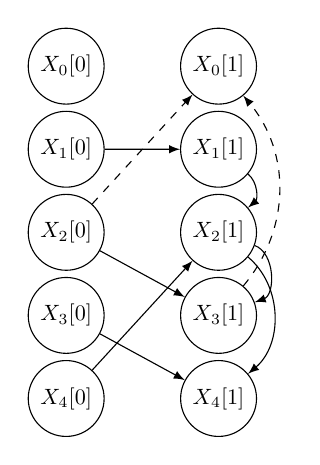
\begin{tikzpicture}[
  node distance=0.1cm and 1.2cm,
  t0/.style={draw,circle},
  t1/.style={draw,circle},
  scale=0.8, transform shape
]

\node[t0] (x00) {$X_0[0]$};
\node[t0,below=of x00] (x10) {$X_1[0]$};
\node[t0,below=of x10] (x20) {$X_2[0]$};
\node[t0,below=of x20] (x30) {$X_3[0]$};
\node[t0,below=of x30] (x40) {$X_4[0]$};

\node[t1,right=of x00] (x01) {$X_0[1]$};
\node[t1,below=of x01] (x11) {$X_1[1]$};
\node[t1,below=of x11] (x21) {$X_2[1]$};
\node[t1,below=of x21] (x31) {$X_3[1]$};
\node[t1,below=of x31] (x41) {$X_4[1]$};

\path
% intra-slice
(x11) edge[-latex, bend left=50] (x21)
(x31) edge[-latex, bend right=40, dashed] (x01)
(x21) edge[-latex, bend left=70] (x31)
(x21) edge[-latex, bend left=50](x41)

% inter-slice
(x30) edge[-latex] (x41) 
(x40) edge[-latex] (x21)
(x20) edge[-latex] (x31)
(x20) edge[-latex, dashed] (x01)
(x10) edge[-latex] (x11)
;

\end{tikzpicture}

\end{document}
